\chapter{場景建立}
\section{前言}
因為這次老師重新規劃了球場及球員的大小、重量......等等,我們重新規劃了整個球場及新建了球員模型,沒有沿用過去的設計。\\
\section{建立球員}
我們使用Onshape重新繪製了球員模型,這次規劃想改變過去bubbleRob看起來較呆版、圓潤的設計,因此設計了一台跑車作為我們的球員。File-Import-Mesh,選擇要匯入的檔案匯入球場,如(圖.\ref{球員建立}) 。接著加入joint\\
加入joint:滑鼠右鍵-Add-Joint-Revolute\\
\
\begin{figure}[hbt!]
\begin{center}
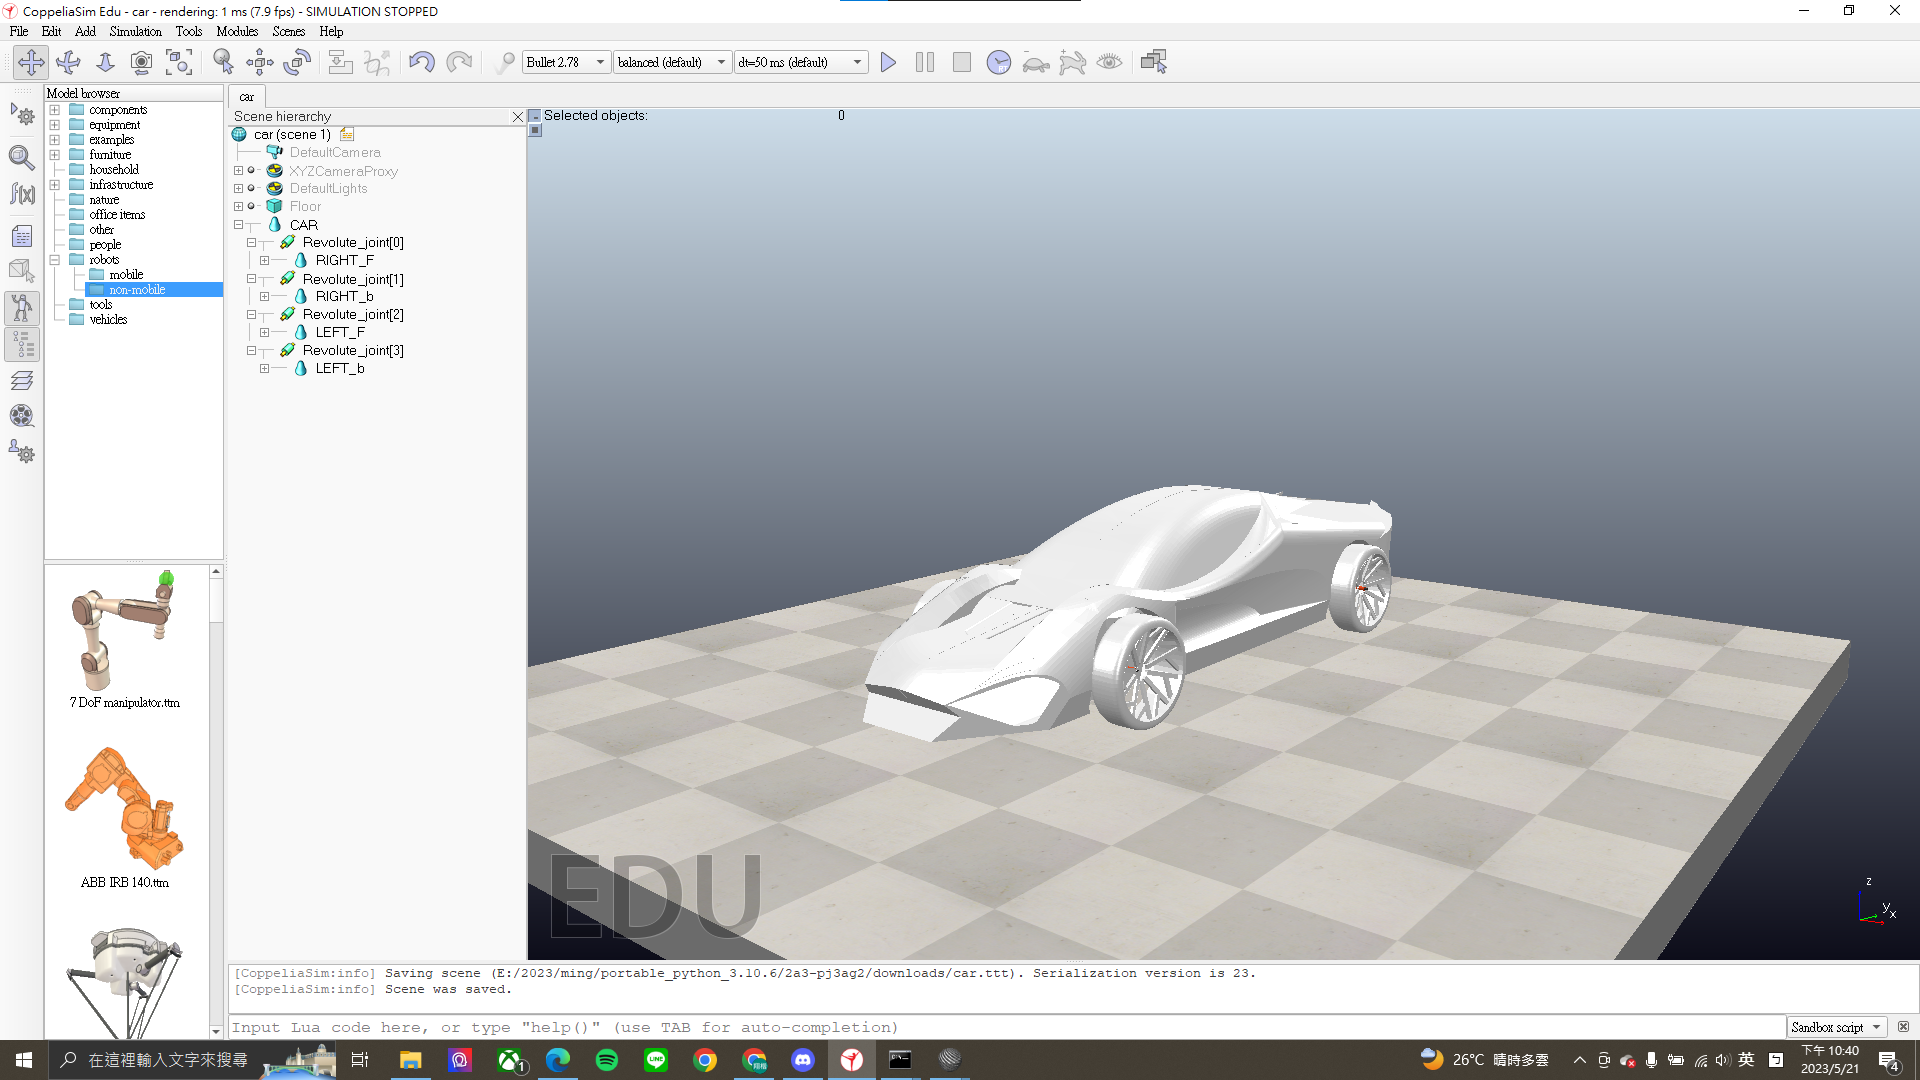
\includegraphics[width=10cm]{球員}
\caption{\Large 球員建立}\label{球員建立}
\end{center}
\end{figure}
\\
\
後發現比例錯誤,因此直接在CoppeliaSim內進行縮小,但因本來設計的跑車高度太低太扁平,可能會有無法推到球的狀況發生,因此不是使用等比縮小,而是直接將各部分拉至規定尺寸。如(圖.\ref{球員建立2})\\
\
比例放大縮小步驟:點選物件左邊圖示-View modify geornrtry-若勾選Keep proportions為進行等比放大,若取消勾選擇可以個別調整大小。\
\begin{figure}[hbt!]
\begin{center}
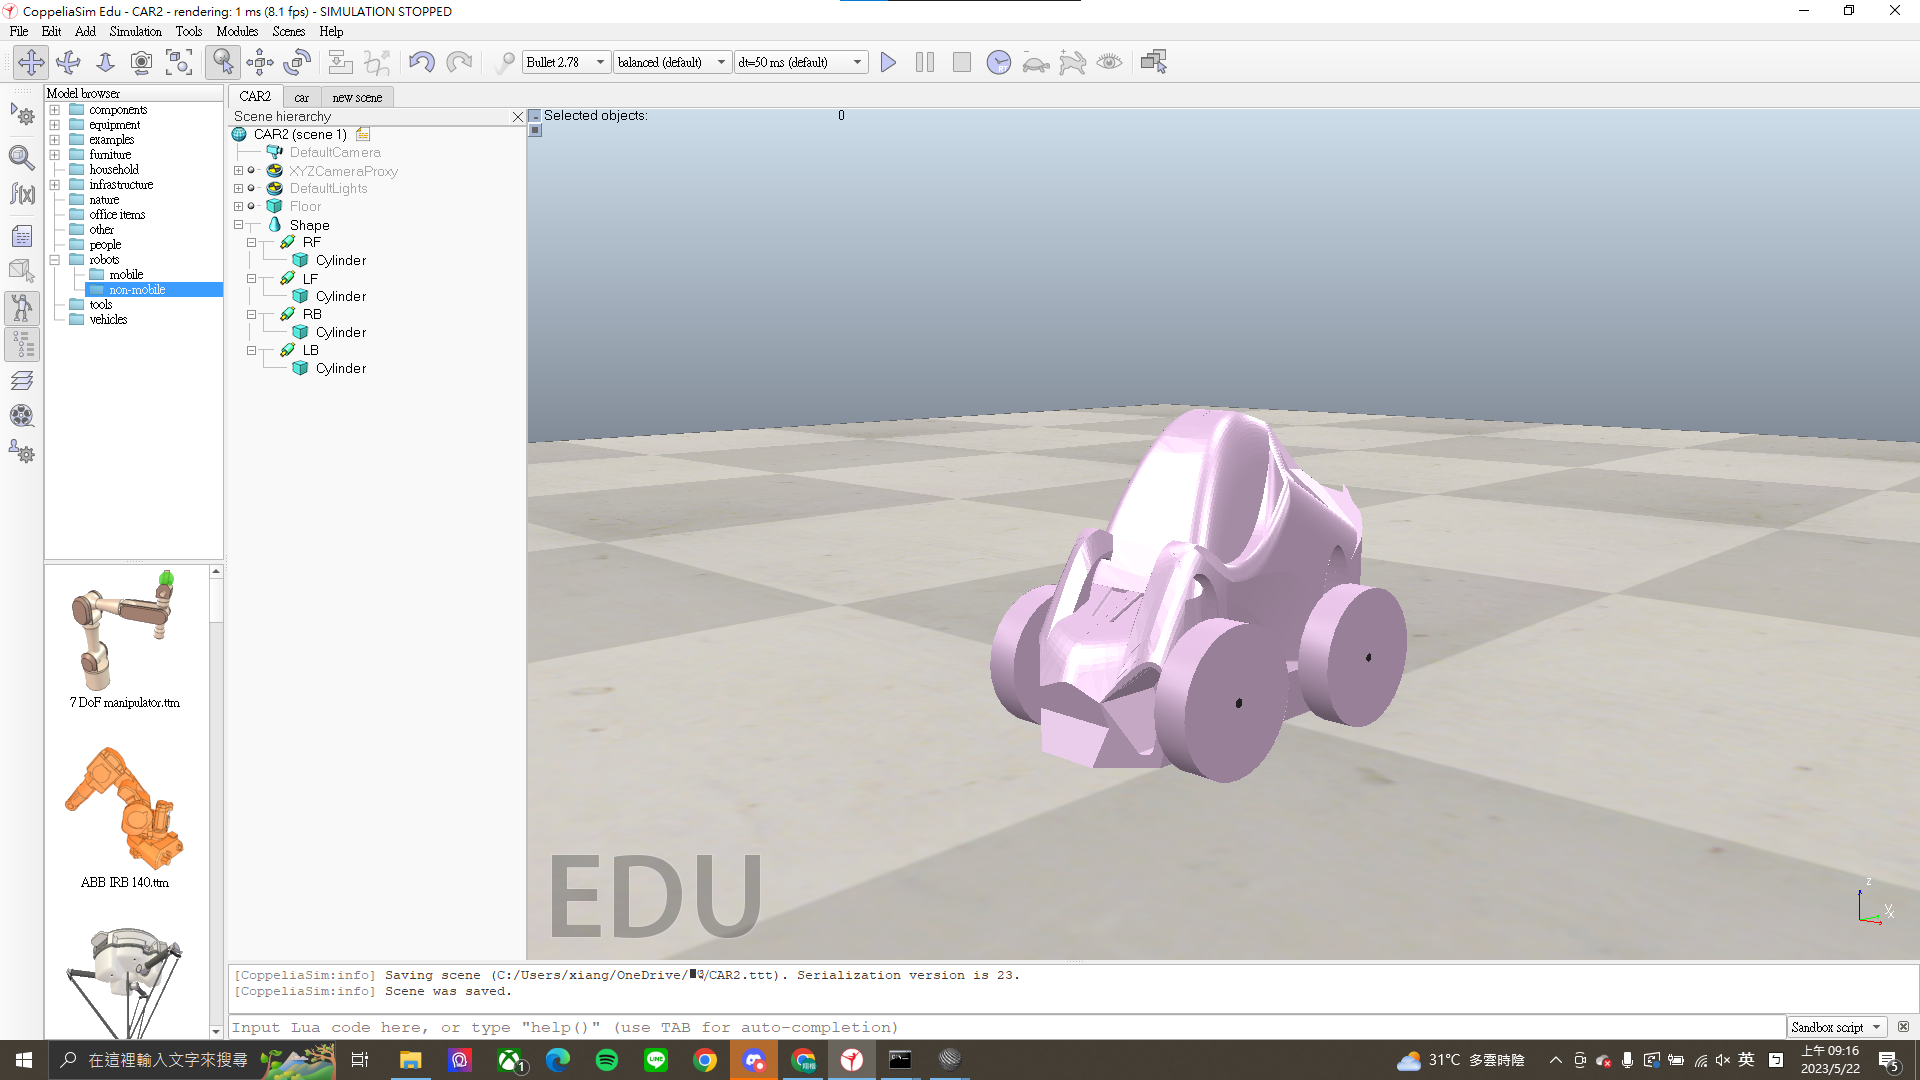
\includegraphics[width=10cm]{球員2}
\caption{\Large 球員建立2}\label{球員建立2}
\end{center}
\end{figure}\
\section{建立記分板}
我們使用Onshape重新繪製了機械式記分板,如(圖.\ref{記分板建立}),接著匯入到CoppeliaSim內進行爆炸拆件,拆件後加入joint如(圖.\ref{匯入記分板})。
\begin{figure}[hbt!]
\begin{center}
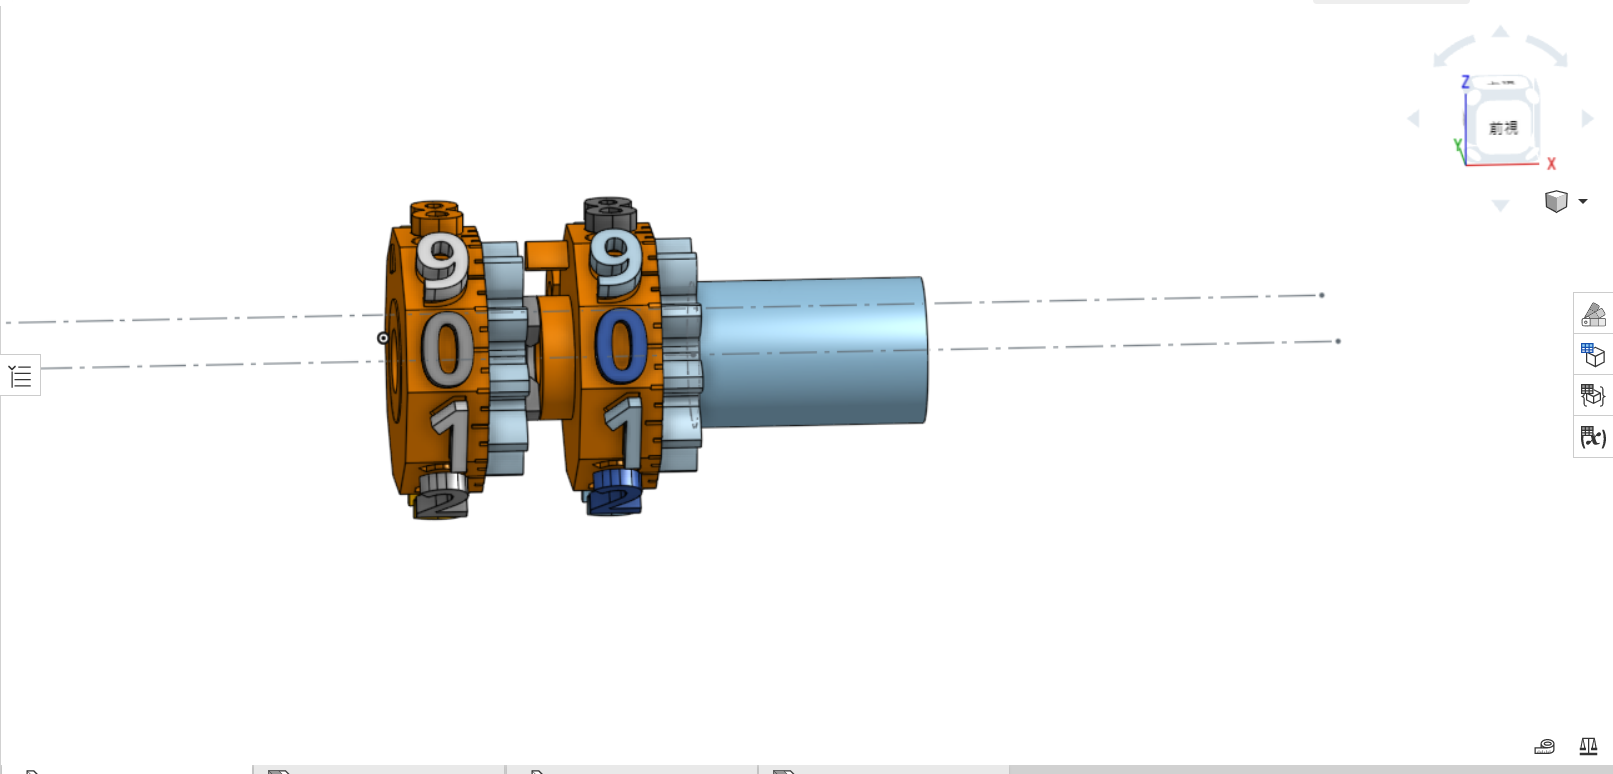
\includegraphics[width=10cm]{螢幕擷取畫面 2023-05-22 092654}
\caption{\Large 記分板建立}\label{記分板建立}
\end{center}
\end{figure}\
\begin{figure}[hbt!]
\begin{center}
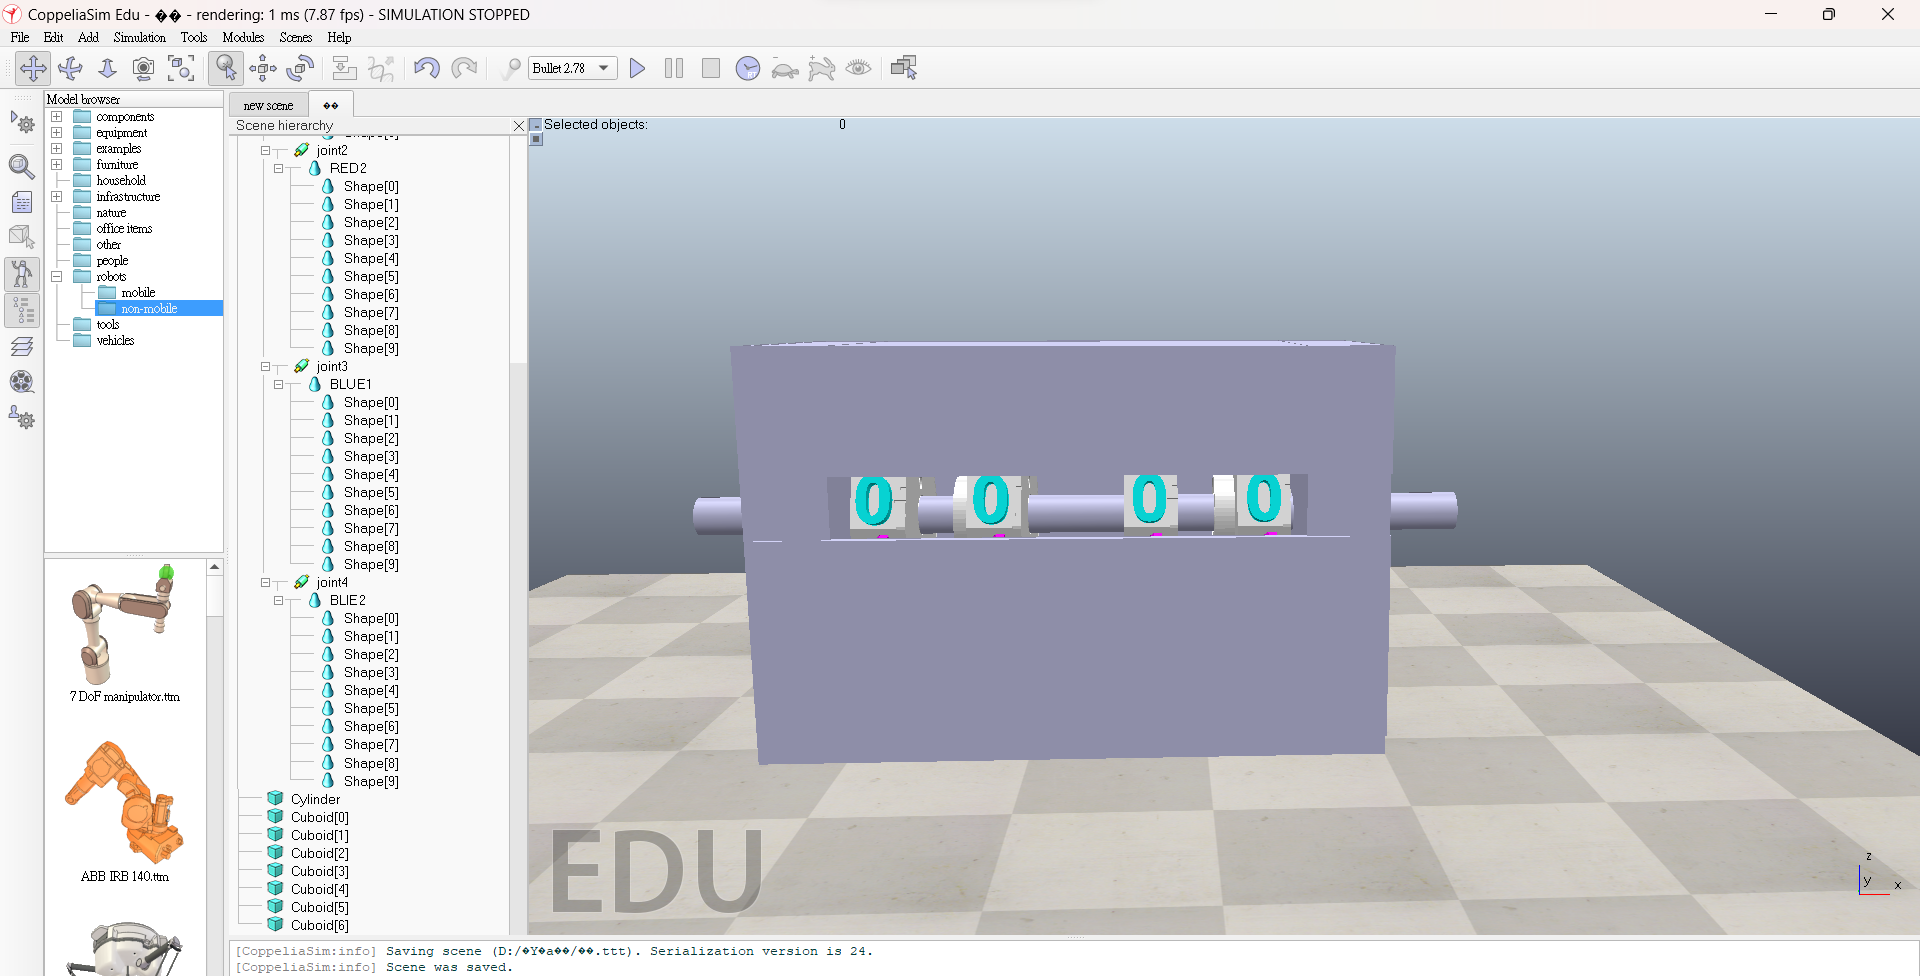
\includegraphics[width=10cm]{螢幕擷取畫面 2023-05-22 093018}
\caption{\Large 匯入記分板}\label{匯入記分板}
\end{center}
\end{figure}\
\newpage
\section{建立球場}
我們使用solidworks繪製了球場底板及球門,如(圖.\ref{球場繪製})、(圖.\ref{球門繪製}),匯入CoppeliaSim後接著建立感測器,如(圖.\ref{建立球場})。\
\begin{figure}[hbt!]
\begin{center}
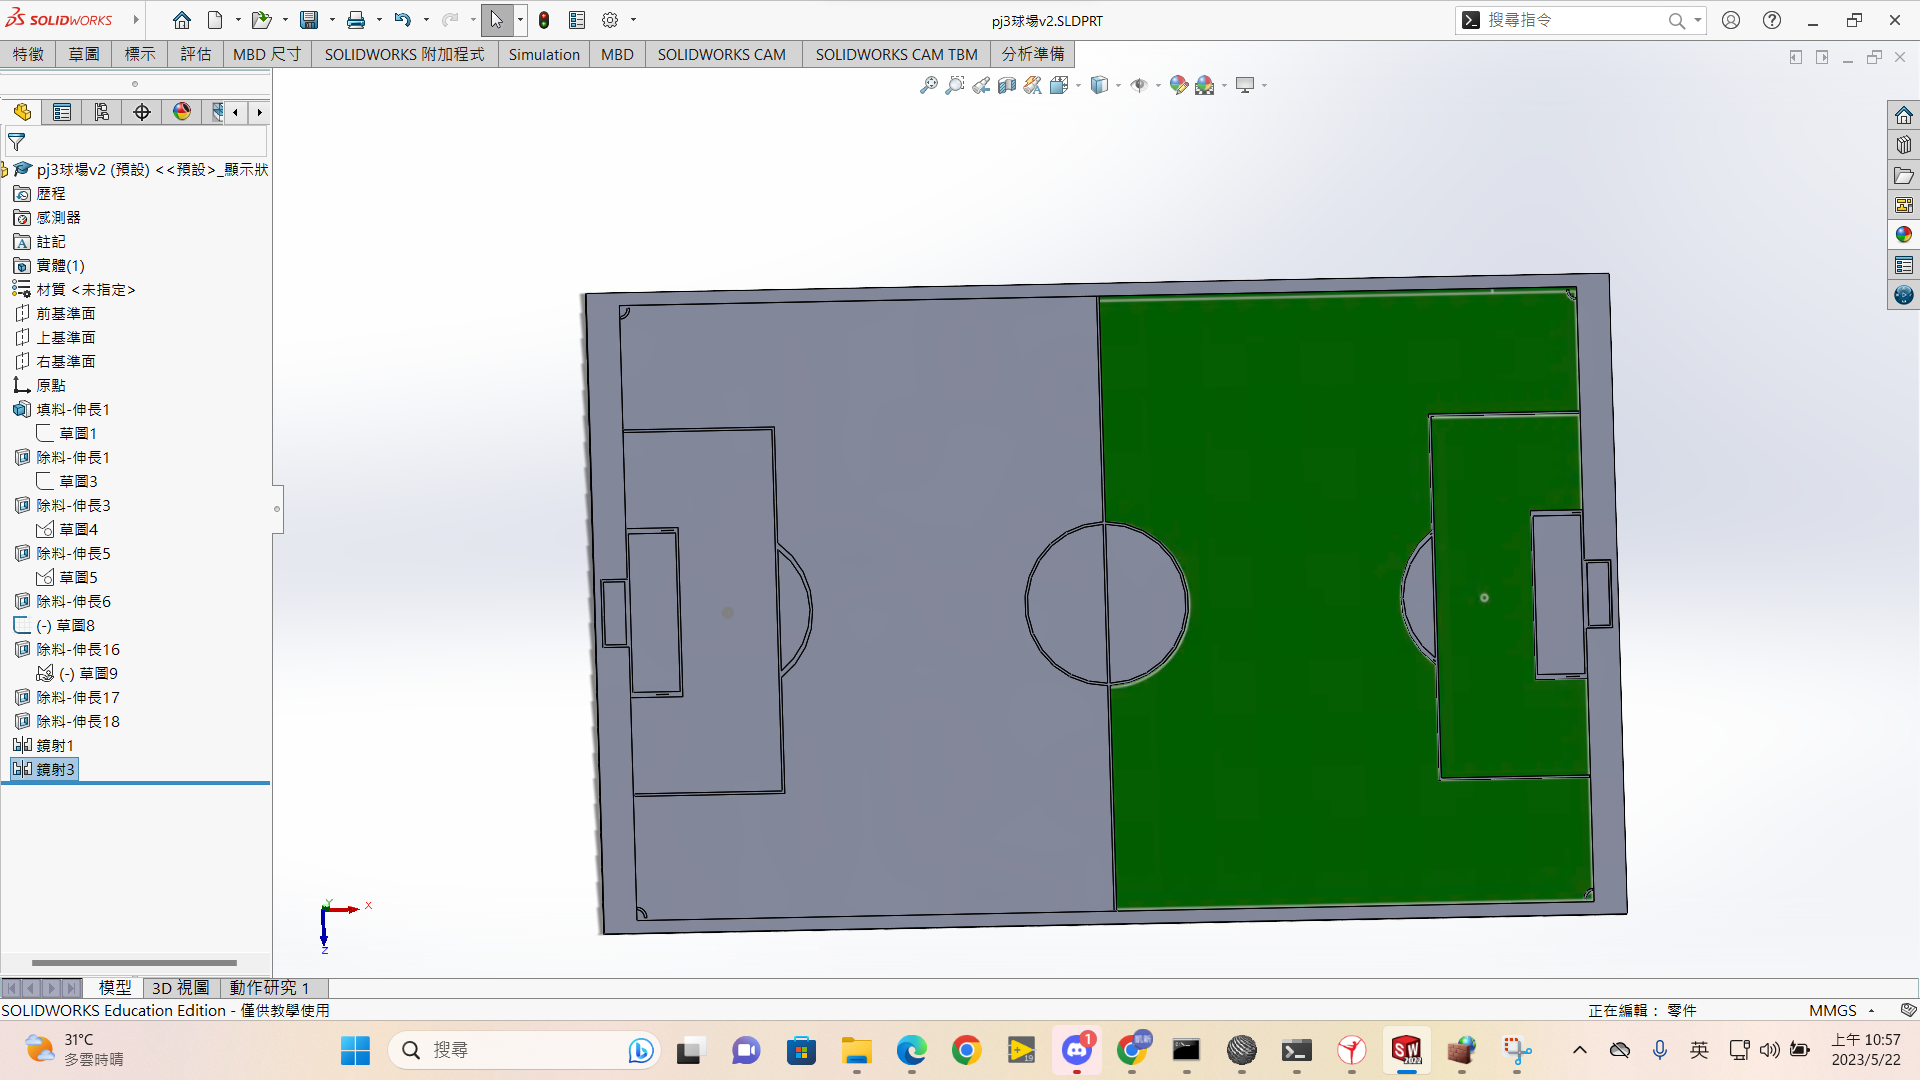
\includegraphics[width=8cm]{螢幕擷取畫面 2023-05-22 105718}
\caption{\Large 球場繪製}\label{球場繪製}
\end{center}
\end{figure}\
\begin{figure}[hbt!]
\begin{center}
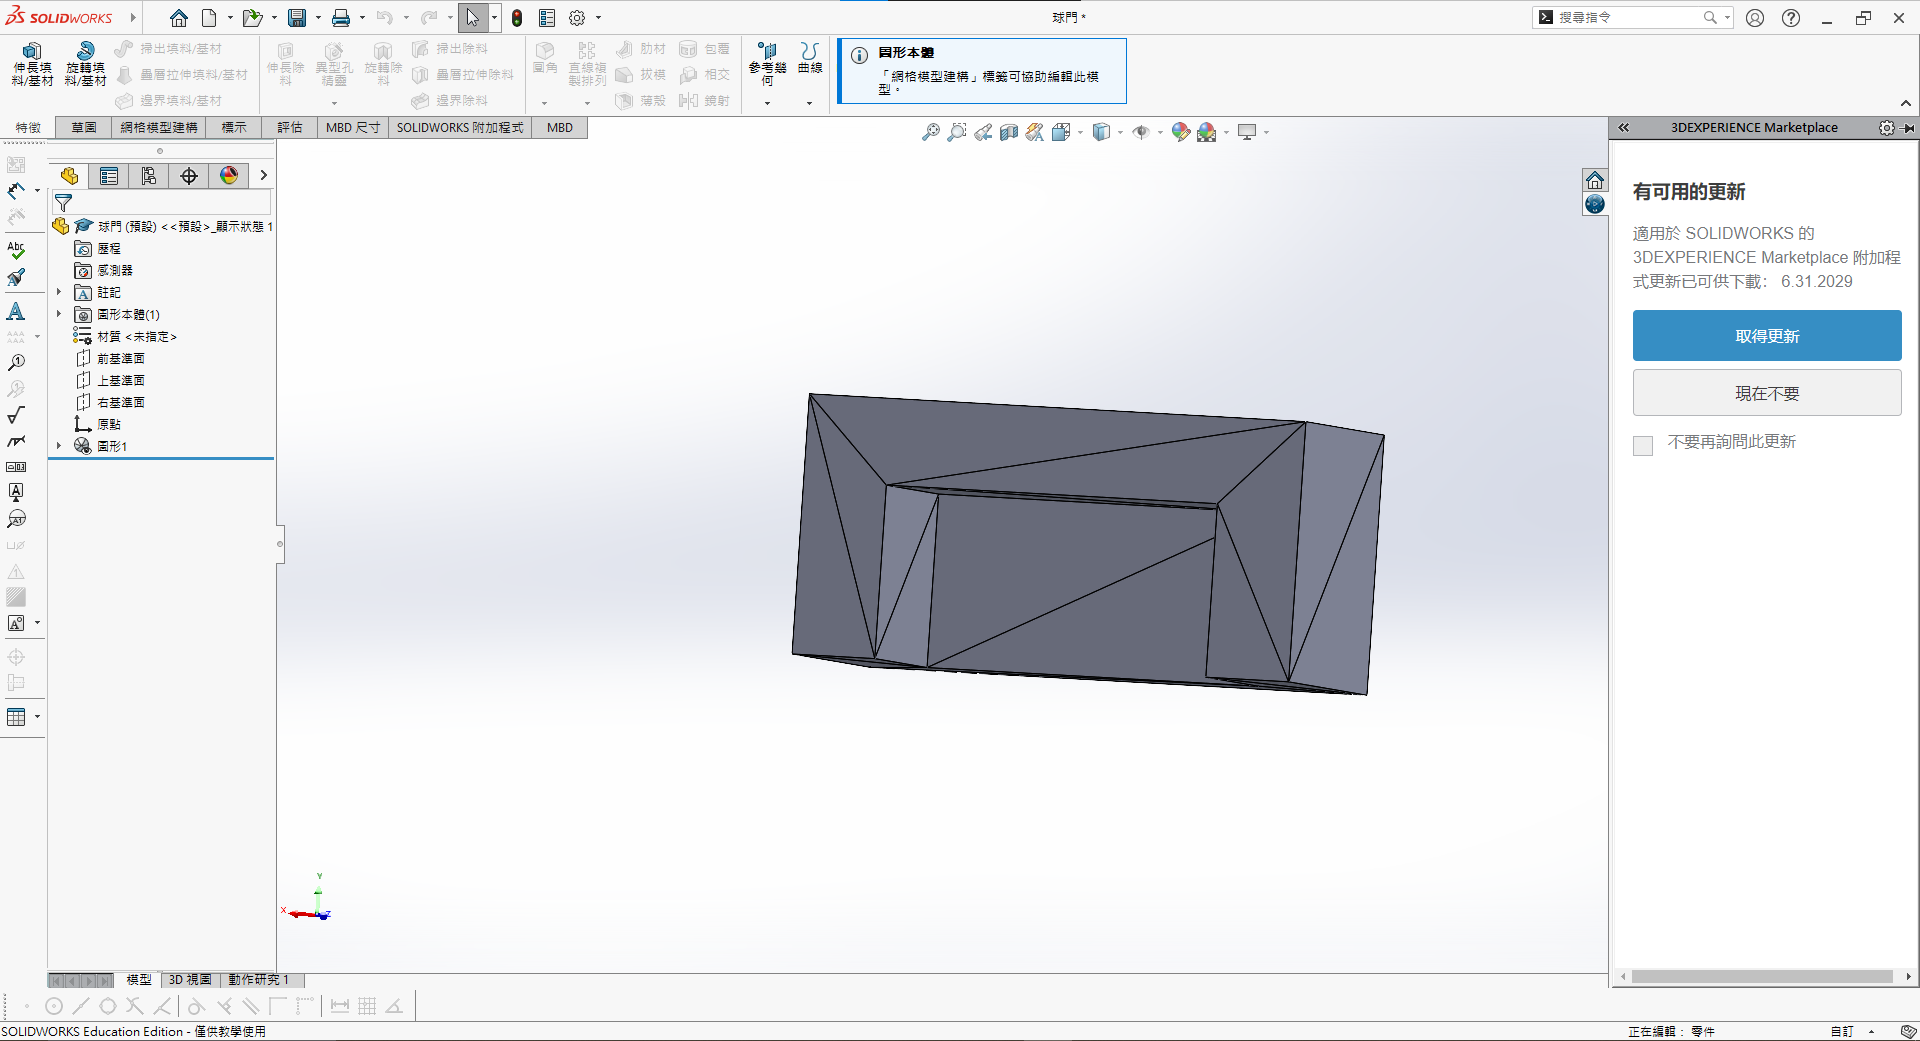
\includegraphics[width=8cm]{球門}
\caption{\Large 球門繪製}\label{球門繪製}
\end{center}
\end{figure}\
\begin{figure}[hbt!]
\begin{center}
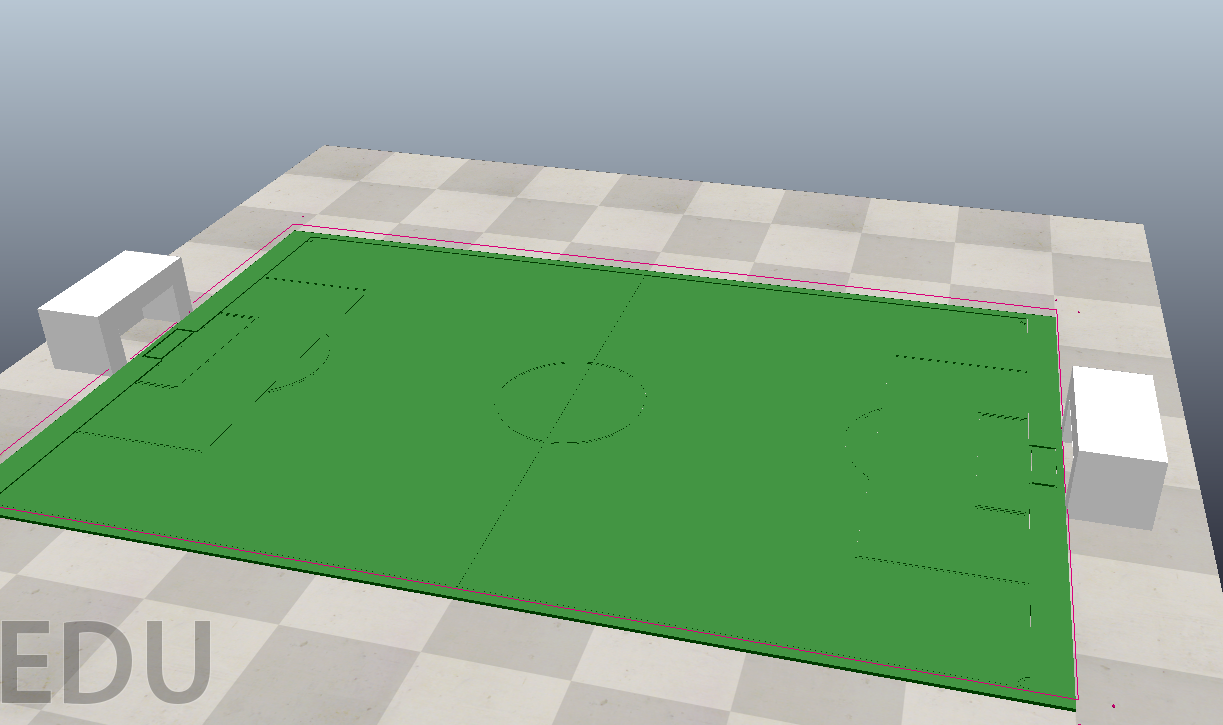
\includegraphics[width=8cm]{螢幕擷取畫面 2023-05-22 101830}
\caption{\Large 建立球場}\label{建立球場}
\end{center}
\end{figure}\
\newpage
\section{整合場景}
接著將所有檔案拉到同一視窗內,球員進行分色,場地位置調整及加入感測器。\\
球員變色:點選本體旁邊圖示-Adjust color-Amibient/diffuse component-拉動RGB調整顏色即可。\\
加入感測器:Add Proximity sensor-Ray type\\
成果如(圖.\ref{場景建立完成})
\begin{figure}[hbt!]
\begin{center}
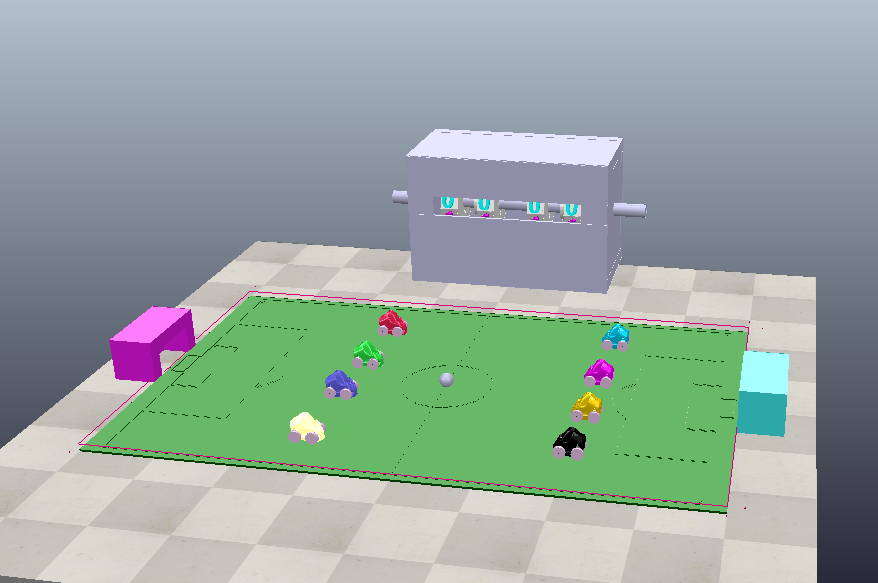
\includegraphics[width=12cm]{螢幕擷取畫面 2023-05-22 105450}
\caption{\Large 場景建立完成}\label{場景建立完成}
\end{center}
\end{figure}\
\newpage